\documentclass[12pt]{article}
\usepackage{../thesis_style}

\title{Chapter 3: Fredholm problem of wave operator on torus}
\date{}

\begin{document}
\maketitle

Having developed some understanding on elliptic operators, we will now turn our focus to a simple non-elliptic problem. Specifically, we will consider the Fredholm problem of the wave operator on the torus. 


\section{Phenomenology} 

\todo{example on euclidean wave operator}

\section{Propagation of singularity} 
\todo{insert discussion + proof sketch of prop of sing theorem}

\begin{ftheorem}[Propagation of singularity] 
    Suppose we have 
    \begin{enumerate}
        \item $P \in \Psi^k_{cl}(\R^n)$ a properly supported operator,
        \item $\sigma_{k}(P) = p - iq$ for real polyhomogeneous symbols $p, q \in S^{k}_{ph}(\R^{2n}; \R^{n})$, 
        \item $A, B, B' \in \Psi^{0}_{cl}(\R^n)$ compactly supported and $q \geq 0 $ on $\WF(B')$, 
        \item for all $(x, \xi) \in \WF(A)$, there exists $\sigma \geq 0$ such that for all $t \in [-\sigma, 0]$
        \begin{align*}
            \exp(-t\sym[\xi]^{1-k}H_p)(x, \xi) \in \ell(B)
        \end{align*}
    \end{enumerate}
    then for all $s, N \in \R$ and $u \in C^\infty(\R^n)$, there exist $C > 0$ such that 
    \begin{align*}
        \norm[Au]_{H^s} \leq C\brac{\norm[Bu]_{H^s} + \norm[B'Pu]_{H^{s - k + 1}} + \norm[u]_{H^{-N}}}. 
    \end{align*}
\end{ftheorem}


\section{Fredholm problem of totally periodic wave operator} 

Let $\S^1 = [0,1] / (0 \sim 1)$ denote the circle and for any $k \in \N$ let
\begin{align*}
\T^k := \underbrace{\S^1 \times \S^1 \times \dots \times \S^1}_{k}
\end{align*}
denote the $k$-dimensional torus. We shall study the totally periodic wave operator, on $M :=  = \T_t^1 \times \T_x^{n}$ given by
\begin{align}\label{eq: d'Alembertian}
    \Box := \p_t^2 - \sum_{j = 1}^{n -1} \p_{x_j}^2
\end{align}
where $(t, x_1, \dots, x_n)$ are the local coordinates on $M$. Note first that $\Box$ is a second order differential (and thus pseudodifferential) operator with \textit{homogeneous} principal symbol given by 
\begin{align*}
    \sigma_2(\Box)(t, x, \tau, \xi) = \xi_1^2 + \xi_2^2 + \dots + \xi_{n}^2 - \tau^2 = \abs{\xi}^2 - \tau^2. 
\end{align*}
Thus, the characteristic set is given by the zero set of the principal symbol (excluding the zero section), i.e. 
\begin{align*}
\Char^2(\Box) = \set{\sigma_2(\Box) = 0} \setminus \set{(t, x, \tau, \xi) \wh \tau = \xi = 0}
\end{align*}
which lies precisely on the `light cone' eminated from every point $(t, x) \in M$, i.e.  
\begin{align*}
\Char^2(\Box) := \set{(t, x, \tau, \xi) \wh 0 \neq \abs{\xi}  = \abs{\tau}} 
\end{align*} 

So, clearly the operator is not elliptic everywhere, and microlocal elliptic estimate does not work on points in $\Char^2(\Box)$.  Instead, we will proceed via the ``complex absorption" method \ref{}. First, we perturb the operator by some operator $Q$ with real non-negative homogeneous principal symbol, namely, 
\begin{align*}
Q := \chi(t)^2 \p_t^2
\end{align*}
where $\chi : \S^1 \to [0, 1]$ is a smooth cut-off satisfying
\begin{align*}
\chi(t) = 
\begin{cases}
1 & t \geq  1 - \delta \text{ or } t \leq \delta \\
0 &  \delta + \delta' < t < 1 - \delta - \delta'
\end{cases}
\end{align*}
where $\delta, \delta' \in (0, 1/8)$ (ensuring that $\delta+ \delta' < 1/4$). 

\begin{center}
    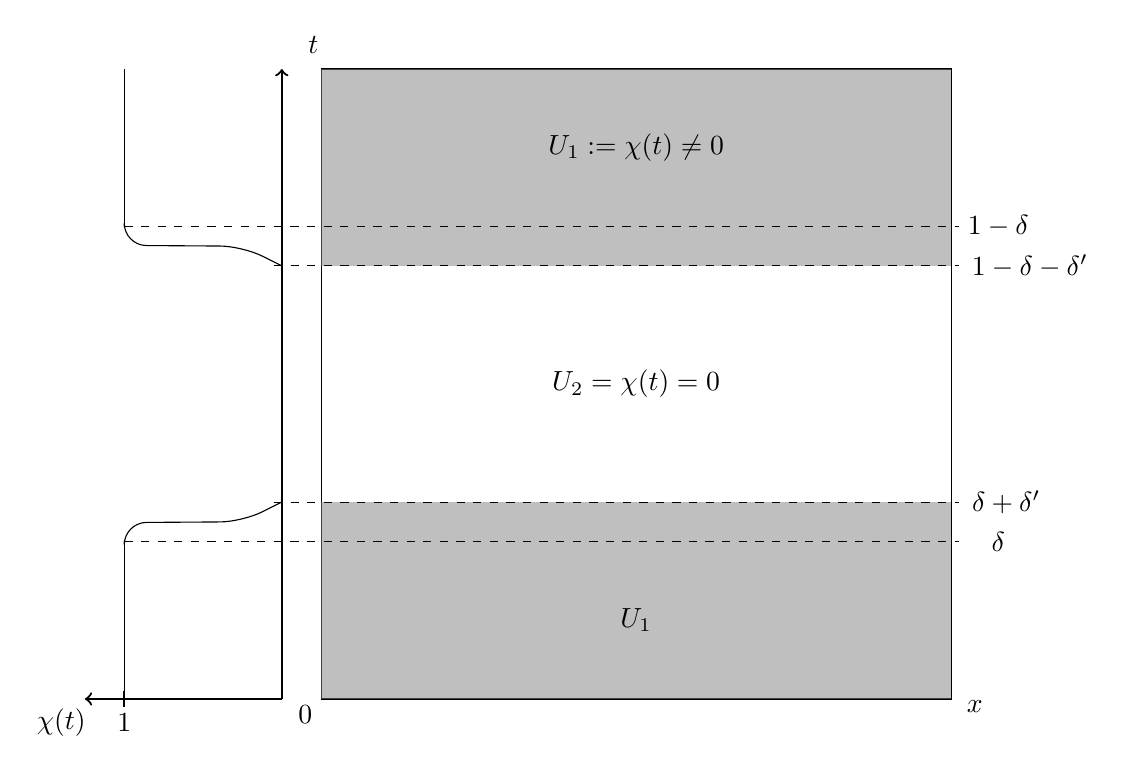
\begin{tikzpicture}
    \draw [] (0, 0) rectangle (8, 8);
    \fill [gray, opacity=0.5] (0, 0) rectangle (8, 2.5);
    \fill [gray, opacity=0.5] (0, 5.5) rectangle (8, 8);
    \draw [dashed] (-2.5, 2) -- (8.1, 2);
    \draw [dashed] (-2.5, 6) -- (8.1, 6);
    \draw [dashed] (-0.6, 5.5) -- (8.1, 5.5);
    \draw [dashed] (-0.6, 2.5) -- (8.1, 2.5);
    \node at (8.6, 2) {$\delta$}; 
    \node at (8.6, 6) {$1 - \delta$};
    \node at (8.7, 2.5) {$\delta + \delta'$}; 
    \node at (9, 5.5) {$1 - \delta - \delta'$};

    
    \node at (8.3, -0.1) {$x$};
    \node at (-0.1, 8.3) {$t$}; 
    \node at (-0.2, -0.2) {$0$};
    \node at (4, 7) {$U_1 :=  \set{\chi(t) \neq 0}$ };
    \node at (4, 1) {$U_1$};
    \node at (4, 4) {$U_2 = \set{\chi(t) = 0}$};
    
    
    \draw [->, thick] (-0.5, 0) -- (-3, 0); 
    \draw [->, thick] (-0.5, 0) -- (-0.5, 8);
    \draw [-, thick] (-2.5, 0.1) -- (-2.5, -0.1);
    \node at (-3.3, -0.3) {$\chi(t)$};
    \node at (-2.5, -0.3) {1}; 
    
    \draw (-2.5, 0) -- (-2.5, 2);
    \draw[rounded corners=8pt] (-2.5, 2) -- (-2.5, 2.24) -- (-1, 2.25) -- (-0.5, 2.5);
    \node at (-2.5, 8) (right start) {};
    
    \draw (-2.5, 8) -- (-2.5, 8 - 2);
    \draw[rounded corners=8pt] (-2.5, 8 - 2) -- (-2.5, 8 - 2.24) -- (-1, 8 - 2.25) -- (-0.5, 8 - 2.5);
    \end{tikzpicture}
\end{center}
We note that $\Box - iQ$ is again a second order differential operator, but its principal symbol changes to 
\begin{align}
\sigma_2(\Box - iQ)(t, x, \tau, \xi) = \abs{\xi}^2 - \tau^2 + i \chi(t) \tau^2. \label{eq: p - iq} 
\end{align}
Therefore, characteristic set of $\Box - iQ$ is given by the zero set of (\ref{eq: p - iq}) minus the 0 section. In $U_2$, where $\chi(t) = 0$, $\sigma_2(\Box - iQ) = 0$ whenever $\abs{\xi} = \abs{\tau}$. On the other hand, outside of $U_2$, $\chi(t) \neq 0 $. Thus, the imaginary part of $\sigma_2(\Box - iQ)$ is zero only if $\tau = 0$ which implies that $\xi = 0$ if the real part were to be zero as well. Thus, $\sigma_2(\Box - iQ) = 0$ in $U_2^c$ only if $\xi = \tau = 0$ which is the zero section excluded from the characteristic set. In short, the characteristic set is given by the close set 
\begin{align*}
\Char^2(\Box - iQ) 
& = \set{\sigma_2(\Box - iQ) = 0} \setminus 0 \\
& = \set{(t, x, \tau, \xi) \wh \chi(t) \neq 0 \text{ and }  0 \neq \abs{\xi} = \abs{\tau}} \subset T^* M \setminus 0. 
\end{align*}

We see now that the pertubation $Q$ introduced an entire region, $U_1$, called the absorption region where $\Box - iQ$ is (microlocally) elliptic. We can then use propagation of singularity estimate to investigate the regularity of solutions to the equation
\begin{align*}
(\Box - iQ) u = f
\end{align*}
for $u, f \in \sch'(\R^n)$. \\

\todo{Mention the sympletic structure on the torus and the Hamiltonian flow $\exp(sH_p)(t, x, \tau, \xi) = (t + s\tau, x + s \xi, \tau, \xi)$. As expected, this is tangential to the characteristic set.}

\begin{fdefinition}
    Let $M$ be the manifold and $\Box -i Q$ be the operator defined above \ref{}. For each $s \in \R$, we define a subspace of $H^{s}(M)$ 
    \begin{align*}
    \chi^s = \set{u \in H^s(M) \wh (\Box - i Q)u \in H^{s - 1}(M)}. 
    \end{align*}
    Together with inner product, 
    \begin{align*}
    \inprod[u, v]_{\chi^s} := \inprod[u, v]_{H^{s}} + \inprod[(\Box - iQ)u, (\Box - iQ)v]_{H^{s -1}}
    \end{align*}
    $\chi^s$ is a Hilbert space. 
\end{fdefinition}



\begin{flemma} \ref{taylorpde}
    Let $T: X \to Y$ be a bounded linear map between Banach spaces $X, Y$ and let $T' : Y' \to X'$ be the dual linear map. Then
    \begin{enumerate}
        \item $\ker T' = T(X)^\perp$. 
        \item If $T$ has closed range, then $T'(Y')  =\ker T'$.  
    \end{enumerate}
\end{flemma}
\begin{proof}
    The dual map is defined by $\inprod[Tx, y] = \inprod[x, Ty]$, where $\inprod $ is the pairing between a Banach space and its dual, $\inprod[x, y] = y(x)$, $x \in X, y \in Y'$. Thus, if $w \in T(X)^\perp$, $w = T(y)$
    \begin{align*}
    \forall y' \in Y, \inprod[y', w] = \inprod[y', Ty] = \inprod
    \end{align*}

\end{proof}


\todo{having already assumed that $\Box - iQ$ has closed range}
\begin{flemma}
    For any $s \in \R$, the maps 
    \begin{align*}
    &\Box - iQ : \chi^s \to H^{s - 1}(M) \\
    &\Box + iQ^* : H^{s - 1}(M)^* = H^{1 -s}(M) \to \brac{\chi^{s}}^*
    \end{align*}
    satisfies 
    \begin{align*}
    \coker (\Box - iQ) \subset \ker (\Box + iQ^*). 
    \end{align*}
\end{flemma}
\begin{proof}
    First note that the element of the cokernel
    \begin{align*}
    \coker (\Box - iQ) = H^{s -1}(M) / (\Box - iQ)(\chi^s)
    \end{align*}
    are precisely the elements $u \in H^{s - 1}(M)$ orthogonal to the image of $\Box - iQ$, i.e. $\inprod[u, v]_{\chi^s} = 0$, $\forall v \in (\Box - iQ)(\chi^s)$. It remains to show that $(\Box + iQ^*)(u) = 0$ for any $u \in  $
    
    \begin{align*}
    \inprod[v, (\Box + iQ^*) u] = \inprod[(\Box - iQ)v, u] = 0. 
    \end{align*}
    
\end{proof}

Our goal is then to prove the following theorem. 
\begin{ftheorem}
    For each $s \in \R$, the operator
    \begin{align*}
    (\Box - iQ): \chi^s \to H^{s - 1}(\T^n)
    \end{align*}
    is Fredholm. 
\end{ftheorem}
\begin{proof}
    The main strategy is to prove the esitmates: $\forall N \in \R$, $\forall u \in \chi^s$, there exist positive real number $C > 0$, such that
    \begin{align} \label{eq : fredholm estimate for wave operator} 
    &\norm[u]_{H^s} \leq C \brac{ \norm[(\Box - i Q)u]_{H^{s - 1}} + \norm[u]_{H^N}} \\
    &\norm[u]_{H^s} \leq C \brac{ \norm[(\Box + i Q^*)u]_{H^{s - 1}} + \norm[u]_{H^N}}. 
    \end{align}
    Note that $(\Box - iQ)^* = \Box + i Q^*$. Also, since $M$ is a compact manifold, \ref{} shows that $H^{s} \hookrightarrow H^{N}$ is a compact inclusion for $N < s$. \todo{proof that this transfer to $\chi^s$ as well}. Then, by \ref{}, these esitmates allow us to conclude that $(\Box - iQ) : \chi^s \to H^{s - 1}$ is indeed a Fredhold operator.     \\
    \\
    Let $N \in \R$, $u \in \chi^s$ be given. We define a cut-off function subordinate to $U_1$, namely
    \begin{align*}
    \chi_1(t, x, \tau, \xi) = \chi(t). 
    \end{align*}
    We note that multiplication by $\chi_1$ act as a $0^{th}$ order pseudodifferential operator. Its wavefront set are points where it is non-zero, i.e. 
    \begin{align*}
    \WF'(\chi_1) = \set{(t, x, \tau, \xi) \wh \chi(t) \neq 0 }. 
    \end{align*} 
    
    The estimates (\ref{}) will follow from both microlocal elliptic regularity \todo{remember to include Vasy's microlocal estimate} \ref{} and propagation of singularity estimate. First, in the absorption region $U_1$ where $\Box - iQ$ is microlocally elliptic, giving us the esitmate: $\exists C > 0$ such that
    \begin{align*}
    \norm[\chi_1 u]_{H^s} \leq C \brac{\norm[(\Box - iQ)u ]_{H^{s - 2}} + \norm[u]_{H^N}}
    \end{align*}
    
     Outside the absorption region, however, (\ref{}) does not apply. We will instead relies on propagation of singularity estimate. The crucial geometric observation is that every light ray eminating from a point in $U_1^c$ can be traced, in both forward and backward direction, to a source in $U_1$. 
     
     
     \begin{center}
         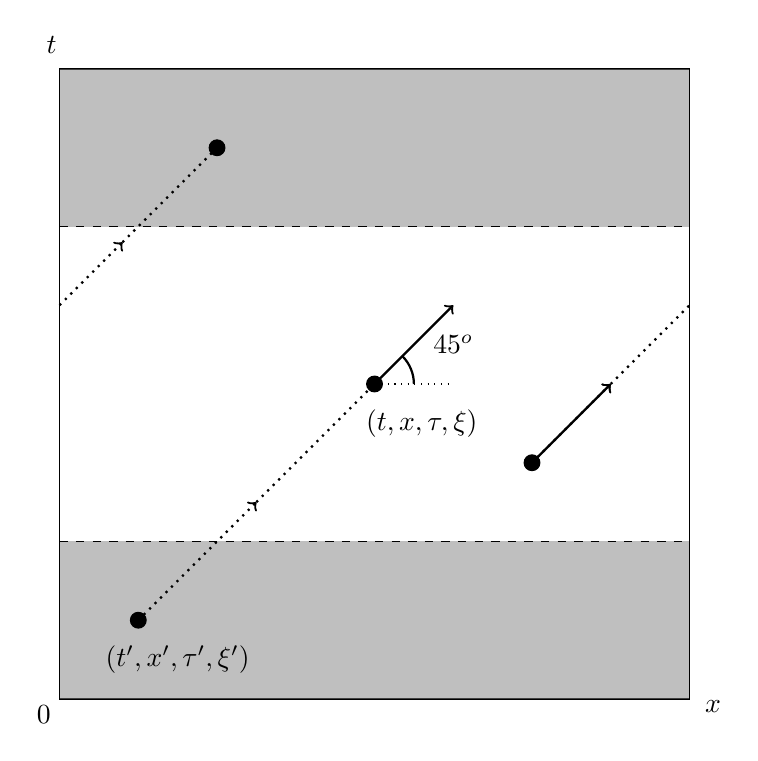
\begin{tikzpicture}
         \draw [] (0, 0) rectangle (8, 8);
         \fill [gray, opacity=0.5] (0, 0) rectangle (8, 2);
         \fill [gray, opacity=0.5] (0, 6) rectangle (8, 8);
         \draw [dashed] (0, 2) -- (8, 2);
         \draw [dashed] (0, 6) -- (8, 6);
         
         \draw [fill=black] (4, 4) circle [radius = 0.1]; 
         \draw [->, thick] (4, 4) -- (5, 5);
         \node at (4.6, 3.5) {$(t, x, \tau, \xi)$}; 
         
         
         \draw [fill=black] (1, 1) circle [radius = 0.1]; 
         \draw [->, thick, dotted] (1, 1) -- (2.5, 2.5);
         \draw [thick, dotted] (2.5, 2.5) --  (4, 4); 
         \node at (1.5, 0.5) {$(t', x', \tau', \xi')$}; 
         
         
         \draw [dotted] (4, 4) -- (5, 4);
         \draw [thick] (4.5, 4) arc (0:45:0.5); 
         \node at (5, 4.5) {$45^o$}; 
         
         \node at (8.3, -0.1) {$x$};
         \node at (-0.1, 8.3) {$t$}; 
         \node at (-0.2, -0.2) {$0$};
         
         
         
        \draw [fill=black] (6, 3) circle [radius = 0.1]; 
        \draw [->, thick] (6, 3) -- (7, 4);
        \draw [->, thick, dotted] (6, 3) -- (7, 4);
        \draw [thick, dotted] (7, 4) -- (8, 5);
        \draw [->, thick, dotted] (0, 5) -- (0.8, 5.8); 
        \draw [thick, dotted] (0.8, 5.8) -- (2, 7); 
        \draw [fill=black] (2, 7) circle [radius = 0.1];
        \end{tikzpicture}
     \end{center}
     
     Therefore, we get the estimate: $\exists C' > 0$
     \begin{align*}
     \norm[u]_{H^s} \leq C' \brac{\norm[\chi_1 u]_{H^s} +  \norm[(\Box - iQ) u]_{H^{s - 1}} + \norm[u]_{H^N} }. 
     \end{align*}
     Substituting \ref{}, we have: $\exists C''> 0$
     \begin{align*}
      \norm[u]_{H^s} 
      & \leq C' \brac{C \norm[(\Box - iQ)u ]_{H^{s - 2}} + C \norm[u]_{H^N} +  \norm[(\Box - iQ) u]_{H^{s - 1}} + \norm[u]_{H^N} } \\
      & \leq C'' \brac{ \norm[(\Box - iQ) u]_{H^{s - 1}} + \norm[u]_{H^N} }
     \end{align*}
     since $\norm[v]_{H^{s - 2}} \leq \norm[v]_{H^{s - 1}}$ for any $v \in H^{s - 2}$. \\
     \\
     Using the same argument, \todo{insert reversing light ray tracing direction} we get a similar estimate for $\Box + i Q^*$, namely,  : $\exists C > 0$
     \begin{align*}
     \norm[u]_{H^s} \leq C \brac{ \norm[(\Box + i Q^*)u]_{H^{s - 1}} + \norm[u]_{H^N}}. 
     \end{align*}
     
     To complete the prove, we 

\end{proof}







\end{document}